%%This is the evaluation part, int includes the following parts.
% <1> Evaluation Metrics, explain the measurements chosen for this experiments
% <2> Test Platform in KNIME, introduced before so we don't really need to repeat it here
% Firstly, we validate our methods and make sure it works for the properties.. Then using the whole data to test the weights tend and also, if it handled the real life data. 
% <3.1> validation part to check the methods work for those situations, but not necessary;; Then big data test to show property to handle those situations. 
% <3> Test Cases Design, the parameters we want to compare, the cases
%   ==> synthetic data
%   ==> Real life data
%   ++ Data to test the property
This chapter presents an experimental evaluation of our repair techniques. At first, we define the evaluation criteria. Next, we briefly introduce the test platforms KNIME and relevant ProM plugins tools. Then, we conduct two kinds of tests. One is based one the demo example proposed in the introduction part, one is on the real life data. 
\section{Evaluation Measurements}
% First talk about our data and our model, then choose the confusion matrix as one measurements. But we should review the traditional measuremtns on process mining before introducing the confusion matrix. but we should also focus on the accuracy part and f-score.
We evaluate repair techniques based on the quality of repaired models with respect to the given event logs. In process mining, there are four quality dimensions generally used to compare the process models with event logs. 
\begin{itemize}
	\item \emph{fitness.} It quantifies the extent of a model to reproduce the traces recorded in an event log which is used to build the model. Alignment-based fitness computation aligns as many events from trace with the model execution as possible.  
	\item \emph{precision.} It assesses the extent how the discovered model limits the completely unrelated behavior that doesn't show in the event log. 
	\item \emph{generalization.} It addresses the over-fitting problem when a model strictly matches to only seen behavior but is unable to generalize the example behavior seen in the event log. 
	\item \emph{simplicity.} This dimension captures the model complexity. According to Occam's razor principle, the model should be as simple as possible.
\end{itemize}
% How to come to confusion matrix?? 
The four traditional quality criteria are proposed in semi-positive environment where only positive instances are available. Therefore, when it comes to the model performance, where negative instances are also possible, the measurement metrics should be adjusted. With labeled traces in the event log, the repaired model can be seen as a binary prediction model where the positive instances are supported while the negative ones are rejected. Consequently, the model evaluation becomes a classifier evaluation. 

% Describe its features and some derived measurements. 
Confusion matrix has a long history to evaluate the performance of a  classification model. A confusion matrix is a table with columns to describe the prediction model and rows for actual classification on data.  The repaired model can be seen a binary classifier and produces four outcomes- true positive, true negative, false positive and false negative shown in the Table \ref{tab:cm}.
\begin{itemize}
	\item True Positive(TP): The execution allowed by the process model has an positive performance outcome.
	\item True Negative(TN): The negative instance is also blocked by the process model.
	\item False Positive(FP): The execution allowed by the process model has an negative performance outcome.
	\item False Negative(FN):The negative instance is enabled by the process model.
\end{itemize} 
% confusion matrix
\begin{table}[]
	\caption{Confusion Matrix}
	\label{tab:cm}
	\begin{tabular}{ll|c|c|}
		\cline{3-4}
		&                   & \multicolumn{2}{c|}{repaired model}                                               \\ \cline{2-4} 
		\multicolumn{1}{l|}{}                                                                         &                   & \multicolumn{1}{l|}{allowed behavior} & \multicolumn{1}{l|}{not allowed behavior} \\ \hline
		\multicolumn{1}{|l|}{\multirow{2}{*}{\begin{tabular}[c]{@{}l@{}}actual \\ data\end{tabular}}} & positive instance & TP                                    & FN                                        \\ \cline{2-4} 
		\multicolumn{1}{|l|}{}                                                                        & negative instance & FP                                    & TN                                        \\ \hline
	\end{tabular}
\end{table}
Various measurements can be derived from confusion matrix. According to our model, we choose the following ones as the potential measurements. 
\begin{itemize}
	\item recall. It represents the true positive rate and is calculated as the number of correct positive predictions divided by the total number of positives.
	\[Recall = \frac{TP}{TP + FN}\]
	\item precision. It describes the ability of the repaired model to produce positive instances.
	\[Precision = \frac{TP}{TP + FP }\]
	%\item specificity. In opposite with recall, it measures the true negative rate.
	%\[Specificity = \frac{TN}{TN + FP}\]
	\item accuracy. It is the proportion of true result among the total number. It  measures in our case how well a model correctly allows the positive instances or disallows the negative instances.
	\[Accuracy = \frac{TP+TN}{TP+TN+FP+FN}\]
	\item F-score is is the harmonic mean of precision and recall.
	\[F_1 = \frac{2*Recall*Precision}{Precision + Recall}\]
\end{itemize}
Generally, there is a trade-off between the quality criteria. So the measurements are only used to compare specific aspects of our techniques.
\section{Experiment Platforms}
KNIME, as a scientific workflow analytic platform, supports automation of test workflow, which helps us repeat experiments efficiently. Yet, traditional evaluation plugins in ProM are not integrated into KNIME, so partial experiments are conducted in ProM.
\subsection{KNIME}
% this section describes how KNIME supports automatic test, FlowVariable and optimization parts of it.
KNIME supports automation of test workflow mainly through the following mechanisms. 
\begin{itemize}
	\item Loop Control Structure. KNIME provides a bunch of control nodes which support re-executing workflow parts.  Nodes representing \emph{Loop Start} appear in pairs with nodes for \emph{Loop Nodes}, the workflow between pairs is executed recursively in a fixed number, or until certain conditions are met. In our test, we repeat our repair techniques for different parameter settings by applying loop structure into KNIME workflow.
	\item Flow Variables. Flow Variables are used inside a KNIME workflow to parameter node settings dynamically. When it combines with loop control structure, tests with different settings is able to conduct automatically.
\end{itemize}
What's more, there are nodes provided by KNIME to optimize the value of some parameters with respect to a cost function. As long as a cost function is provides, KNIME is able to automatically optimize any kind of parameters. 
\subsection{ProM Evaluation Plugins}
%Here we discuss the plugins to test other aspects of our methods. 
Although KNIME offers a powerful approach to conduct experiments, the integration of traditional process mining evaluation plugins into KNIME is out of our capability due to the time limits. To evaluate repaired models with traditional metrics, we use an existing ProM plugin called \textbf{\emph{Multi-perspective Process Explorer}} \cite{mannhardt2015multi}. This plugin accepts  Petri net and an event log as inputs, and gives out fitness, and precision measurements which are based on the traditional alignment conformance checking. 
\section{Experiment Results}
\subsection{Test on Demo Example}
In this experiment, we aim to answer the question: Will our repair method overcome shortcomings of current techniques which are shown in the introduction chapter?  

% for situation 1, we can not get the ideal model, the reason is that we can not keep the model like just as it states, we can 

\subsection{Comparison To Other Techniques}
This section represents some situations where current repair techniques can't handle properly, while our algorithm gives out an improved repaired model. 

\emph{Situation 1}, unfit part!! added subprocess are too much!! Where the addition of subprocesses and loops are allowed, while the structure changes are impossible, 
Fahrland's method applies the extension strategy to repair model by adding subprocesses and loops in the procedure. It introduces unseen behavior into the model. However, if the behaviors which are already in the model is unlikely to be removed from the model. One simple example is shown in the following part. 

Dee's method is based on Fahrland's method. Deviations are calculated at first and used to build subprocesses for model repair. However, before building subprocesses, it classifies the deviations into positive and negative ones with consideration of trace performance. Only positive deviations are applied to repair model. Different to Fahrland's method, it improves the repaired model performance by limiting the introduced subprocesses. Still, it can't get rid of the defect mentioned before. 

\emph{Situation 2}, For fitted data in the model, can not recognize them!! where overlapped data noise can not be recognized, trace variant with more negative effect is treated as positive and kept in the model, which we should delete them.   
% Here we want to give an example of the overlapped data, compared to IM rediscoverty, easy.. But for Dees' method, firstly, they have labeled data; The analyzed the deviations of them, but when one deviation dominates, then the tree can not see the others. Some data are ignored..

\emph{Situation 3}, with long-term dependency!! fitted part or new added part!! none of the current techniques can handle this problem yet.
Simple examples listed, but will this repeat the last section?? 


% Conclusion part
For one exclusive choices, 
but with long-term dependency detected and added in the model, precision and accuracy increase, since model with long-term dependency blocks the negative information by adding transitions and places to limit activity selection. 

\subsection{Test On Real life Data}
% here we will list all the data here but before describe the test data
We choose a publicly available event log from BPI challenge 2015 as our user cases and compare current repair techniques on it. 
\subsubsection{Data Description}
The data set for BPI Challenge 2015 contain 5 event logs which are provided by five Dutch municipalities respectively. Those event logs describe the building permit application around four years. We choose it as our user cases due to the following reasons.
\begin{itemize}
	\item The event logs hold attributes as potential KPIs to classify traces. Attribute \textbf{SUMleges} which records the cost of the application is a candidate to label traces as positive or negative if its value  is over one threshold. What's more, we can take the throughput time of the application as another potential KPI. \\
	In a word, this data set provides us information to reasonably label traces.
	\item The five event logs describe an identical process, but includes deviations caused by the different procedures, regulations in those municipalities. Also, the underlying processes have changes over four years.\\
	So, this data set gives us a basic process but also allows deviations of the actual event logs and predefined process, which builds the environment for repair techniques.
\end{itemize}
Firstly, we conduct our experiments on event log called \textbf{BPIC15\_1.xes.xml}. This event log includes 1199 cases and 52217 events. But the event classes for those events are  with the sum of 398. So we preprocess the event log and get a proper subset of data as our user case. 

We filter the raw event log by \textbf{\emph{Filter Log By Simple Heuristic}} in ProM with the following setting. 40 for the start, end  activities and the events between them, at end. We get the event log $D1$. After this, we calculate the throughput time for each trace and add it as a trace attribute \textbf{throughput time}. 
Then we classify traces according to  \textbf{SUMleges} and  \textbf{throughput time} separately. When our performance goal is to reduce the cost of application, if \textbf{SUMleges} of one trace is over 0.7 of the whole traces, this trace is treated as negative, else as positive. The similar strategy is applied on the attribute \textbf{throughput time}. A trace with \textbf{throughput time} higher than 0.7 of all traces is considered as a negative instance. Following this preprocess, we have event logs in Table \ref{tab:event-log} available for our tests. 
\begin{table}	
	\caption{Test event log from real life data BPI15-1}
	\label{tab:event-log}
	\begin{tabular}{|l|l|l|l|l|}
		\hline
		Data ID & Data Description                                & Traces Num & Events Num & Event Classes \\ \hline
		D1      & \makecell{Heuristic filter  \\ with 40 }                     & 495        & 9565       & 20             \\ \hline
		D2      & \makecell{Apply heuristic filter \\ on D1 with 60      }     & 378        & 4566       & 12            \\ \hline
		D3.1    & \makecell{classify on SumLedges;  \\ values below 0.7 as positive} & 349        & 6744       & 20             \\ \hline
		D3.2    & \makecell{classify on SumLedges;  \\ values above 0.7 as negative }& 146        & 2811       & 20             \\  \hline
		D3.3    & union of D3.1 and D3.2                             & 495        & 9596       & 20             \\ \hline
		D4.1    & \makecell{ classify on throughput time;  \\ values below 0.7 as positive} & 349        & 6744       & 20             \\ \hline
		D4.2    & \makecell{classify on throughput time;  \\ values above 0.7 as negative} & 146        & 2811       & 20            \\ \hline
		D4.3    & union of D4.1 and D4.2                             & 495        & 9596       & 20           \\ \hline
	\end{tabular}
\end{table}

Based on the filtered data, we derive corresponding Petri nets as reference process models. The Table \ref{tab:ref-models} lists the models with different setting. \textbf{IM-infrequent} is one variant of Inductive Miner working on event logs with infrequent traces. \textbf{Noise} is set as the threshold to filter out infrequent traces. After mining a reference model, we compare them with  corresponding event logs to get the basis lines for later evaluation.
% should we explain the data and the model, they are different with old files!!
% Please add the following required packages to your document preamble:
% \usepackage{multirow}
\begin{table}[h]
	\caption{Generated reference models for test}
	\label{tab:ref-models}
	\resizebox{\textwidth}{!}{
	\begin{tabular}{|llll|lllllllll|}
		\hline
		\multirow{2}{*}{\thead{Model\\ ID}} & \multirow{2}{*}{\thead{Used \\Data}} & \multirow{2}{*}{\thead{Setting}}  &  
		\multirow{2}{*}{\thead{Event\\Class}} & \multicolumn{8}{c}{\thead{CM Evaluation}}                     \\ 
		\cline{5-13}
		&                                                                           &                                                                             &                                                                            &Data & TP & FP & TN & FN & recall & precision & accuracy & F1 \\ \hline
		M1                                                                      & D1                                                                        & \makecell[l]{IM-infrequent: \\ Noise Setting: 20} & 20                                                                         & D3.3 & 112   & 40   & 106   & 237   & 0.321       &0.737           &   0.440       &   0.447 \\
		
		&                                                                      & &                                                                          & D4.3 & 131   &  21  &  128  & 215   & 0.379       & 0.862           & 0.523          & 0.526    \\
		
		\hline
		M2                                                                      & D1                                                                        & \makecell[l]{IM-infrequent: \\ Noise Setting: 50} & 20                                                                         & D3.3 & 106   & 39   &  107  & 243    & 0.304        &  0.731         &0.430          &0.429    \\
		
		&                                                                      & &                                                                          & D4.3 & 125   &   20 & 129   &221    &    0.361    & 0.862           & 0.513          &0.509    \\
		\hline
		
		M3                                                                      & D2                                                                        & \makecell[l]{IM-infrequent: \\ Noise Setting: 20} & 12                                                                         &D3.3 &  0  & 0   & 146   & 349   & 0       &NaN           &    0.295      & 0   \\
		
		&                                                                      & &                                                                          & D4.3 &  0  & 0   & 149   & 346   & 0       & NaN           &  0.301        &0    \\
		\hline 
		
		M4                                                                      & D2                                                                        & \makecell[l]{IM-infrequent: \\ Noise Setting: 50} & 12                                                                         &D3.3 &  0  &  0  &  146  & 349   & 0       & NaN           &     0.295     & 0\\   
		&                                                                      & &                                                                          & D4.3 &  0  & 0   & 149   & 346   & 0       & NaN           &  0.301        &0    \\
		
		\hline
	\end{tabular}
 }
\end{table}
As seen in table above, the reference models don't apply well to the corresponding event logs. So changes on the models are in demand, to reflect better the reality and also to enforce the positive instances and avoid negative instances. 

\subsubsection{Test Result}
% we don't need to transfer page to landscape view, because we have many rows too.
We conduct experiments in the following types.
\begin{itemize}
	\item \textbf{Type 1} Inductive Miner only on the positive event log to discover a model. The default setting with infrequent variant and noise threshold as 20 is chosen. Later, the mined model is checked on the labeled event with positive and negative instances. This method is abbreviated as IM.
	\item \textbf{Type 2} Repair Model from \cite{fahland2015model} is applied on the positive event log to discover a model. The default setting is chosen. Later, the mined model is checked on the labeled event with positive and negative instances. This method is abbreviated as Fahland, named after the name of main author.
	\item \textbf{Type 3} The method proposed from our thesis, is applied on the labeled event log with positive and negative instances. Default setting  for the control parameters is 1.0 while the parameters to generate Petri nets from directly-follows graph are set as the same as experiment Type 1.  Later, the repaired model is evaluated on the labeled data. This method is abbreviated as Dfg.
\end{itemize}
Those types are applied on event log groups of {D3.1,D3.2,D3.3} and {D4.1,D4.2,D4.3} listed in Table \ref{tab:event-log} and models from Table \ref{tab:ref-models}. The experiment result is shown in the Table \ref{tab:result}. 

	\begin{table}[h]
		\centering
		\caption{Test Result on BPI15-M1 data}
		\label{tab:result}
		\resizebox{\textwidth}{!}{
		\begin{tabular}{lll|llllllll|ll}
			\hline
			\multirow{2}{*}{\thead{event \\ log}} & \multirow{2}{*}{\thead{reference \\ model} }                &    \multirow{2}{*}{\thead{method}}       & \multicolumn{8}{l}{ \thead{confusion matrix metrics}}                              & \multicolumn{2}{|l}{\thead{traditional metrics}} \\
			\cline{4-13}
			 &  &     &
			  \thead{TP}  & \thead{FP} & \thead{TN}  & \thead{FN}  & \thead{recall} & \thead{precision} & \thead{accuracy} & \thead{F1}   & \thead{fitness}           & \thead{precision}           \\
			  \hline
			D3.1      & M1,M2,M3,M4              & IM & 137 & 48 & 118 & 289 & 0.32   & 0.74      & 0.43     & 0.45 & ?                 & ?                   \\
			D3.1      & M1              & Fahland   & 343   & 136  &10     &6     &0.983        & 0.716           &   0.713       & 0.829     &        ?           &         ?            \\
			
			D3.3      & M1              & dfg       &  124   &  52  &  94   &    225 &   0.355     &     0.705      & 0.44         & 0.472      & ?                   &             ?        \\
			
			\hline
			D3.1      & M2              & Fahland   & 317    & 133   &   13  & 32    &  0.908      &    0.704       & 0.667         &  0.793    &      ?             &     ?                \\
			
			D3.3      & M2              & dfg       & 124    &   52 &   94  & 225    &  0.355      &   0.705        &  0.44         &  0.472    &                   &                     \\
			
			\hline
			D3.1      & M3              & Fahland   & 349    & 145   &  1   &  0   &  1.0      &   0.706        &   0.707       &  0.828    &                   &                     \\
		
			D3.3      & M3              & dfg       &  0   &   0 &  349   &  146   &  0      &   NaN        &  0.295        &   0   &                   &                     \\
			\hline
			
			D3.1      & M4              & Fahland   &  271   & 107   &  77   &  39   & 0.779       &   0.718        &   0.628       &  0.747    &      ?             &          ?           \\
			
			D3.3      & M4              & dfg       &  0   &  0  &   349  &  146   &   0     &      NaN     & 0.295         &    0  &           ?        &    ?                 \\
		\hline
			D4.1      & M1              & IM &  131   &  21  & 128    &  215   &    0.379    & 0.862           &   0.523       &    0.526  &           ?        &      ?               \\
			D4.1      & M1              & Fahland   &  325   &  133  &  16   & 21    &   0.939     &  0.710         &  0.689       & 0.808     &                   &                     \\
			
			D4.3      & M1              & dfg       &  139   & 36   & 113    &   207  &   0.402     &   0.794        &   0.509       &   0.534   &                   &                     \\
			\hline
			D4.1      & M2              & Fahland   & 325    &  130  & 19    &  21   & 0.939       &    0.714       &  0.695        &  0.811    &                   &                     \\
		
			D4.3      & M2              & dfg     &  139   & 36   & 113    &   207  &   0.402     &   0.794        &   0.509       &   0.534   &                   &                     \\
			\hline
			D4.1      & M3              & Fahland   & 87    &  29  & 120    &  259   & 0.251       &    0.75       &  0.418        &  0.377    &                   &                     \\
		
			D4.3      & M3              & dfg       &  0   &  0  & 346    &  149   &  0      &   NaN        &   0.303       &  0    &                   &   \\ 
			\hline
			D4.1      & M4              & Fahland   & 63    &  20  & 129    &  283   & 0.182       &    0.759       &  0.388        &  0.294    &                   &                     \\
		
			D4.3      & M4              & dfg       &   0  & 0   &  346   & 149    &   0     &    NaN       &     0.303     &  0    &                   &   \\    
			 \hline              
		\end{tabular}}
	\end{table}

With the similar measurements, it is observed that the repaired models from \textbf{Type 2} are more complex that Dfg method. One example is given for the tests of M1 on event log D4.1 for \textbf{Type 2} and M1 on event log D4.3. 
\begin{figure}[htp]
	\centering
	\begin{subfigure}[b]{0.48\textwidth}
		\centering
		\includegraphics[width=0.5\linewidth, height=0.7\textheight]{figures/evaluation/PN-result-D5-3-M1-fahland.pdf}
		\caption{repaired model with techniques in \cite{fahland2015model}}
		\label{fig:model_fahland}
	\end{subfigure}%
	\begin{subfigure}[b]{0.48\textwidth}
		\centering
		
\includegraphics[width=0.5\linewidth, height=0.7\textheight]{figures/evaluation/PN-result-D5-3-M1-dfg-1-1-1.pdf}
		\caption{repaired model with }
		\label{fig:model_dfg}
	\end{subfigure}
	\caption{example for situation 1 where $M_{1.1}$ is repaired by adding subprocess in the form of loops, which results in lower precision compared with the expected model $M_{1.2}$.}
	\label{fig:model_change_1}
\end{figure}



Due to the different settings in our method, forces from the reference model, positive, and negative event logs are balanced differently during repair, which results in different process models. To investigate the effect of those setting on the repaired model, we repeat our experiments on the following setting. 

Each of three control parameters for the existing model, positive and negative instances changes value from 0.0 to 1.0 with step 0.1. With this setting, directly-follows relation is generated. Afterward, the default setting of Inductive Miner Infrequent with noise threshold 20 is used to mine Petri nets from the generated directly-follows graph. 


So in total, we conduct over thousand experiments to investigate our methods. Based on those results, we draw plots to show the tendency of evaluation results on the parameters for the existing model, positive and negative event logs. 

\begin{figure}
	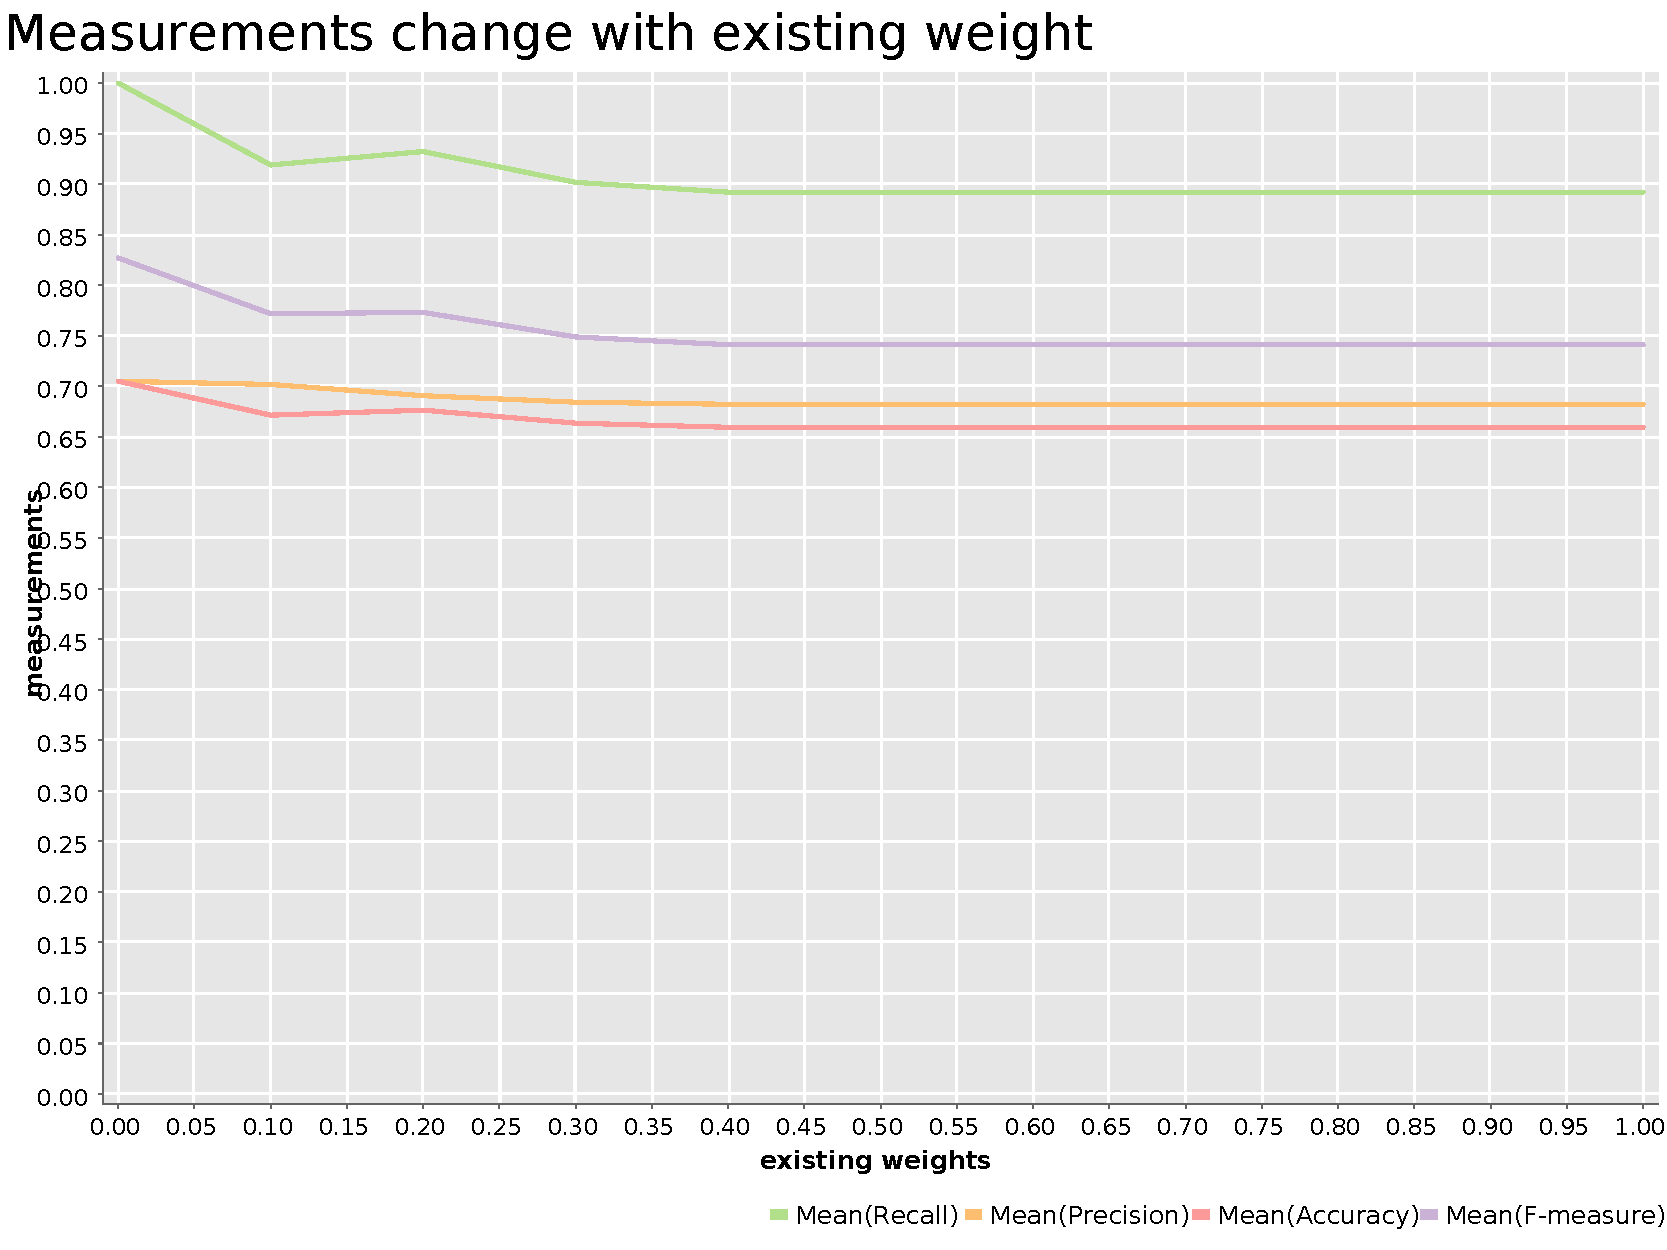
\includegraphics[width=\linewidth]{figures/evaluation/M3-D43-ext-weight-plot.pdf}
	\caption{result with control parameter for existing model on event log D3.3 and model M3}
	\label{fig:ext-weight}
\end{figure} 
From the Figure \ref{fig:ext-weight}, with the parameter for the existing model going up, recall goes up while accuracy and precision goes down. The reason behind it is possibly ????.


\begin{figure}[h]
	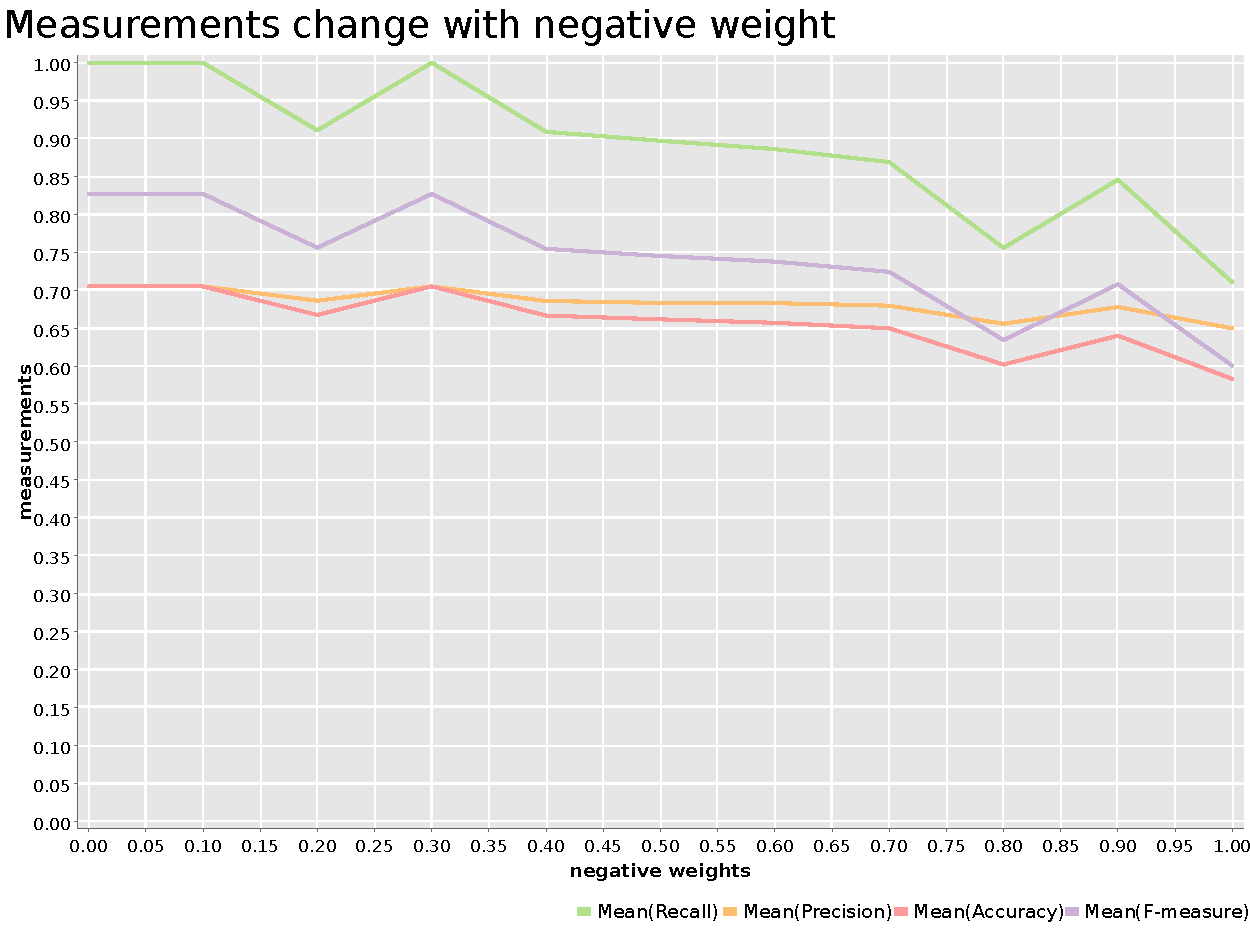
\includegraphics[width=\linewidth]{figures/evaluation/M3-D43-neg-weight-plot.pdf}
	\caption{result with control parameter for negative instance on event log D3.3 and model M3}
	\label{fig:neg-weight}
\end{figure}
Figure \ref{fig:neg-weight} shows that if the parameter for negative event log increases, precision and accuracy go up. By addressing negative force, our techniques tend to block behavior which leads to low performance output. However, if the negative force is over the force from positive event log and the existing model, certain behavior which contributes to positive performance will also be deleted from the models. In contrast, this creates a model with less recall. 


\begin{figure}[h]
	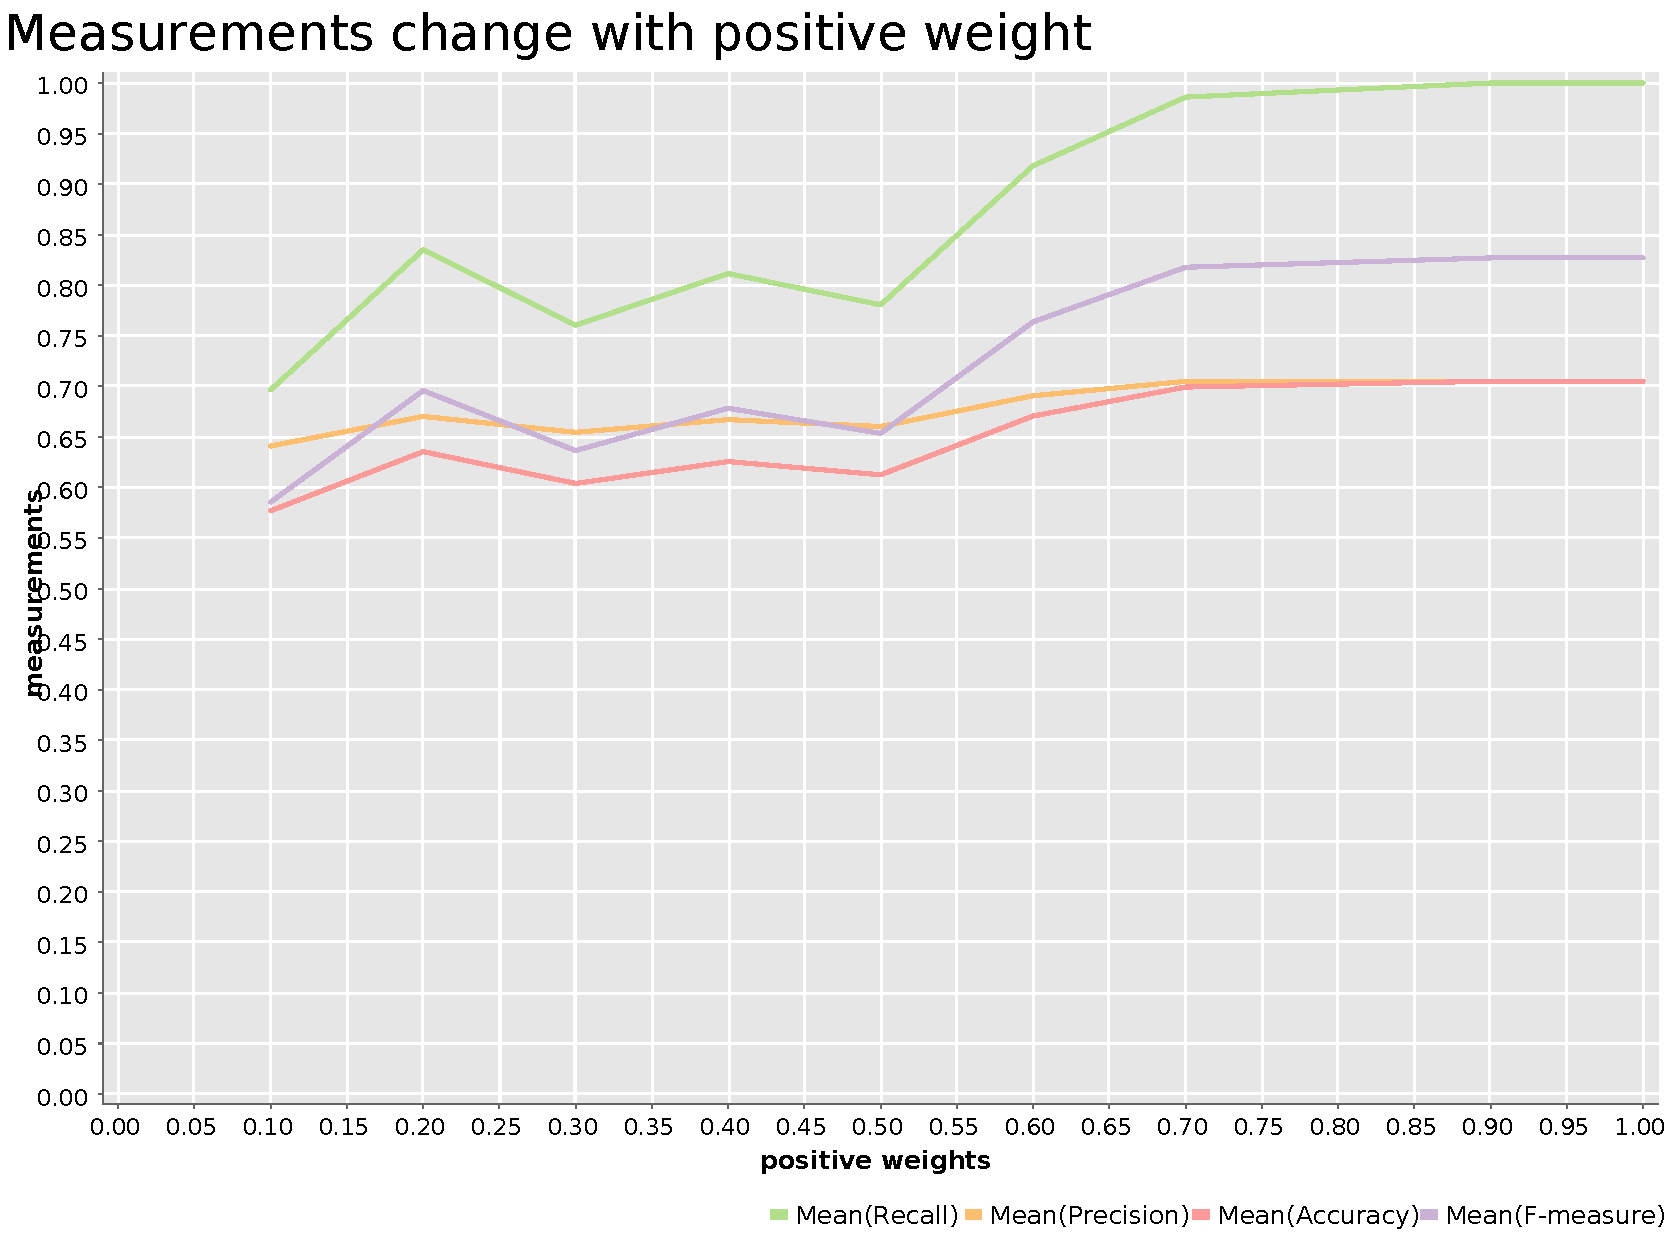
\includegraphics[width=\linewidth]{figures/evaluation/M3-D43-pos-weight-plot.pdf}
	\caption{result with control parameter for positive instance on event log D3.3 and model M3}
	\label{fig:pos-weight}
\end{figure}
Figure \ref{fig:pos-weight} displays the tendency with the parameter for positive event log. When the positive parameter rises, the recall increases. Precision and accuracy also increases but with ???.